\documentclass[letterpaper, 10 pt, conference]{ieeeconf}  % Comment this line out if you need a4paper
\IEEEoverridecommandlockouts
\overrideIEEEmargins                                      % Needed to meet printer requirements.

%\usepackage{graphics} % for pdf, bitmapped graphics files
%\usepackage{epsfig} % for postscript graphics files
%\usepackage{mathptmx} % assumes new font selection scheme installed
%\usepackage{times} % assumes new font selection scheme installed
%\usepackage{amsmath} % assumes amsmath package installed
%\usepackage{amssymb}  % assumes amsmath package installed
%\usepackage{amsthm}
%\usepackage[style=ieee]{biblatex}
%\addbibresource{references.bib}
%
%%\theoremstyle{definition}
%%\newtheorem{definition}{Definition}[section]

%\usepackage{amssymb}
%\usepackage{graphicx}
%\usepackage{epstopdf}
%\usepackage{amsmath}
%\usepackage{subfigure}
%\usepackage{multirow}
%\usepackage{pbox}
%\usepackage{algorithm}
%\usepackage{algpseudocode}
%\usepackage{bm}
%\usepackage{url}


%%%%%%

%\documentclass[conference]{IEEEtran}
%
\usepackage{graphicx}
\usepackage{amsmath}
\usepackage{mathrsfs}
\usepackage{array}
\usepackage{enumerate}
\DeclareMathOperator*{\argmin}{arg\,min}
\DeclareMathOperator*{\argmax}{arg\,max}
\usepackage{amssymb}
\usepackage{mathtools}
\usepackage{breqn}
\usepackage{algorithm}
\usepackage{algorithmic}
\usepackage{varwidth}
%\usepackage{subcaption}
%\usepackage[noend]{algpseudocode}
\makeatletter
\def\BState{\State\hskip-\ALG@thistlm}
\makeatother


\newcommand\NB[1]{$\spadesuit$\footnote{NB: #1}}
\newcommand\RP[1]{$\clubsuit$\footnote{RP: #1}}

\newcommand*{\Z}{\mathbb{Z}}
\newcommand*{\N}{\mathbb{N}}
% reference package for bibtex

%\usepackage{biblatex}
%\addbibresource{mybibliography.bib}

%\usepackage[
%backend=biber,
%style=numeric,
%sorting=ynt
%]{biblatex}

%\addbibresource{mybibliography.bib}


% correct bad hyphenation here
\hyphenation{op-tical net-works semi-conduc-tor}


\begin{document}
%
% paper title
% Titles are generally capitalized except for words such as a, an, and, as,
% at, but, by, for, in, nor, of, on, or, the, to and up, which are usually
% not capitalized unless they are the first or last word of the title.
% Linebreaks \\ can be used within to get better formatting as desired.
% Do not put math or special symbols in the title.
%\title{Using Hidden Markov Models to Improve Autonomous Vehicle Decision Making - Problem Formulation}
%\title{A Hidden Markov Models-based Approach for Automotive Predictive and Assistive Control}
\title{\LARGE \bf A Hidden Markov Model-based Approach for Predictive and Assistive Control in Semi-Autonomous Vehicles}
\author{Rahul Peddi and Nicola Bezzo%
\thanks{Rahul Peddi and Nicola Bezzo are with the Department of Systems and Information Engineering and the Charles L. Brown Department of Electrical and Computer Engineering, University of Virginia, Charlottesville, VA 22904, USA. Email: {\tt \{rp3cy, nb6be\}@virginia.edu}}
%\thanks{$^{2}$Esen Yel is with the Department of Systems and Information Engineering, University of Virginia, Charlottesville, VA 22904, USA. Email: {\tt ey3un@virginia.edu}}
}



%\author{\IEEEauthorblockN{Rahul Peddi$^1$ and Nicola Bezzo$^{1,2}$} 
%\IEEEauthorblockA{
%\small
%$^1$Department of Systems and Information Engineering\\
%\small
%$^2$Department of Electrical and Computer Engineering\\
%\small
%University of Virginia\\
%Email: \{rp3cy, nbezzo\}@virginia.edu}}
%\hyphenation{u-sing}


\maketitle

% As a general rule, do not put math, special symbols or citations
% in the abstract
\begin{abstract}
 Semi-autonomous and autonomous vehicles have been changing the way our roads work...
\end{abstract}
\NB{abstract should present the problem with a little motivation and the approach with the technique and briefly mention the results}
% no keywords




% For peer review papers, you can put extra information on the cover
% page as needed:
% \ifCLASSOPTIONpeerreview
% \begin{center} \bfseries EDICS Category: 3-BBND \end{center}
% \fi
%
% For peerreview papers, this IEEEtran command inserts a page break and
% creates the second title. It will be ignored for other modes.
\IEEEpeerreviewmaketitle



\section{Introduction}
% no \IEEEPARstart

%    Over the last few years, semi-autonomous and autonomous vehicles have become increasingly popular, but they have not replaced traditional vehicles entirely just yet. This leads to a hybrid environment; one that features vehicles of all levels of autonomy. Many of these vehicles to be equipped with some form of adaptive cruise control (ACC) or advance driver assistance systems (ADAS), both of which help the driver make safe decisions while operating the vehicle. These types of systems are forms of human-robot interaction. ACC performs actions autonomously and works at the command of a human who determines a target velocity and a safe following distance. ADAS, on the contrary, acts as an information system for human drivers. These systems, however, are limited in their capabilities as they require constant monitoring from the driver and are unable to predict if the driver will enter a dangerous situation in the future. In addition, these systems can fail to guarantee safety in rapidly transitioning environments.
    
    
%    Because these dangerous situations can occur so rapidly \NB{need citation here}, there is a need to increase the ability to guarantee safety when developing new systems \NB{what do you mean with new systems?} for human drivers. This can be done by increasing the ability to predict and adapt to what will happen in the future. A simple depiction of a danger situation is shown in Fig. \ref{fig:hiway}. \NB{figure needs improvements}

%\NB{I'll go back to this later...intro needs a lot of attention!}
 
%\NB{In a not far future, multiple vehicles with different level of autonomy will have to coexist and operate safely. Examples of such vehicles include cars, vessels, aerial vehicles. Different levels of autonomy are available 1 to 5 for cars, hobby  }   

%\NB{Semi-autonomous and autonomous vehicles are finding their way in our society rapidly. Although new advancements in sensing and autonomy are increasing safety by assisting drivers with line changing warning and assisted braking, } 
\NB{here let's talk about the trolly problem and mention that we see humans as disturbance in this work! discuss about teleoperated robotics that is still big and assistive automation}

Semi-autonomous and autonomous vehicles are finding their way in our society rapidly. As these vehicles proliferate the roadways, we get a mixed environment, meaning that different levels of autonomy are available. Although new advancements in sensing and autonomy are increasing safety by assisting drivers with systems such as adaptive cruise control (ACC) \cite{acc} or advanced driver assistance systems (ADAS) \cite{adas}, these systems are far from perfect. ACC performs actions autonomously and works at the command of a human who determines a target velocity and a safe following distance. ADAS, on the other hand, acts as an information system for human drivers. These systems, however, are limited in their capabilities as they require constant monitoring from the driver and are unable to predict if the driver will enter a dangerous situation in the future. In addition, these systems can fail to guarantee safety in rapidly transitioning environments \cite{accfail}.
    

\begin{figure}[ht]
    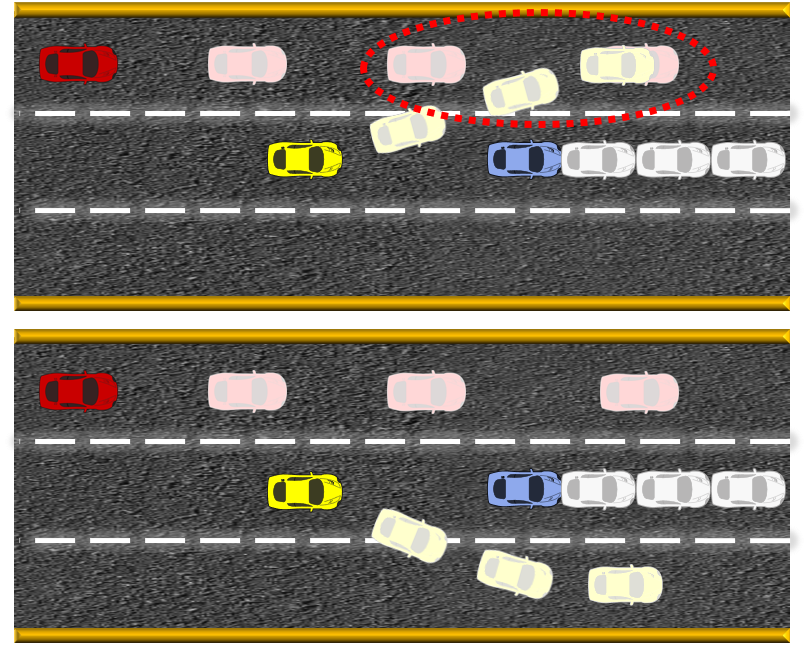
\includegraphics[width=0.48\textwidth]{highway.png}
    \caption{Two possible actions on a highway, where one leads to a dangerous situation in the future(top), and another minimizes risk (bottom)}
    \label{fig:hiway}
\end{figure}
    
    An example of such environment is a large multi-laned area with multiple vehicles. In Fig.\ref{fig:hiway}, a user is driving a vehicle (yellow car) behind a slower vehicle (blue car). In this case, both actions presented in Fig.\ref{fig:hiway} may appear safe to a driver at the moment, but as can be seen by the red circle, one of the lane changes is considerably riskier in the future, because a rapidly approaching vehicle (red car) will enter the same space as the user's vehicle. In this case, we see the driver's actions as potentially adversarial, or as a disturbance, and want to assist the driver. In order to prevent a riskier action from taking place, we are interested in predicting future states of other surrounding vehicles, assessing risk of collisions given the user's actions, and intervening and assisting the driver accordingly. This type of work can be approached as a type of Markov Chain, and we leverage Hidden Markov Model (HMM) theory as well, both of which are commonly used models for many cyber-physical systems (CPS).
    
     In this work, we aim to provide
    \begin{itemize}
    \item{a prediction method that can effectively and efficiently estimate the future positions of surrounding agents}
    \item{an adaptive framework that determines the adjustment of a user's actions and severity of such adjustment that should be made at any point in time}
    \end{itemize}
  
    
    The rest of this paper is organized as follows: in Section \ref{sec:relatedwork}, we discuss related work, and in Section \ref{sec:probform}, we formally define the problem. The general approach is discussed in Section \ref{sec:approach}. In Section \ref{sec:fmwk}, we discuss the specifics of the HMM-based framework, and how it is used to build models. We then use that framework to make online predictions in Section \ref{sec:ahmmpredupdate}, and show how we can fit the models to a system we are observing in Section \ref{sec:omf}. This is followed by a discussion of we use the framework, along with the predictions and fitting, to assist the user in Section \ref{sec:adapt}. Then we demonstrate our results with MATLAB simulations in Section \ref{sec:sims}. Lastly, we discuss our conclusions and future work in Section \ref{sec:concs}.

    
% You must have at least 2 lines in the paragraph with the drop letter
% (should never be an issue)

\section{Related Work} \label{sec:relatedwork}

The study of semi-autonomous and autonomous vehicles has been growing in recent years. As these options have become more available to the average consumer, driving environments have become more mixed, and researchers approach such environments from different viewpoints; those of improving the knowledge about the environment (i.e. prediction) and those that involve controlling for such environments (i.e. autonomy).

The authors in \cite{mpc} use velocity predictions derived from artificial neural networks and GPS systems for Model Predictive Control (MPC), which is presented as a highly complicated optimization problem, and the predictions are only evaluated for one vehicle at a time. The authors in \cite{velnn} and \cite{veldatadriv} take a data science approach and use large data-sets, along with very specific traffic information, in order to make predictions. The use of a Hidden Markov Model based approach for prediction is done in \cite{lanhmm}, where the authors develop an approach treating a vehicle as a hybrid state system to predict the trajectory of a certain behavior. This is done, while assuming knowledge of multiple In \cite{woohmm}, motivated by previous work in HMMs, the authors discuss using a simplified form of the hybrid state system with an HMM to improve lane change prediction scalability over multiple vehicles. In our work, we consider the problem of predicting future velocity and when lane changes are expected by leveraging the theories presented in \cite{mpc} and \cite{woohmm}. 

In terms of controlling vehicles in such environments, the authors in \cite{qmdp} use a Point-Based Markov Decision Process (QMDP) to estimate dangerous situations and react with the appropriate autonomous driving behavior in single-lane situations. The QMDP process employs a robust, but computationally intensive value iteration algorithm in order to do this. In \cite{predcost}, the authors present a prediction and cost-based (PCB) control strategy for autonomous vehicles given a known set of predicted scenarios. In this vein, \cite{vfh+} and \cite{vfh*} discuss reliable obstacle avoidance methods given that obstacle locations and characteristics are known based on artificial physics methods. In \cite{takeover}, with a human-factors based approach, the authors show multiple ways take-over requests can be generated in partially autonomous vehicles, including performance based and environment based characteristics. In our work, we leverage the idea of taking over from \cite{takeover}, along with the theories in \cite{vfh*} to control for future unsafe scenarios we detect in our predictions.

    
\section{Problem Formulation} \label{sec:probform}
 
In this work we are interested in finding an approach to proactively guarantee safety (i.e., something bad will never happen) in multi-vehicle systems operations. We focus on manned vehicles employing an hybrid autonomy scheme as defined in \cite{} in which the control authority is shared between the human and the on-board computer. For the sake of brevity we denote this class of vehicles as {\em hybrid autonomous vehicles} (HAVs), In our scheme, the on-board computer is used as a supervisory monitor to predict and assess safety and assist by correcting undesired human behaviors that may lead to unsafe situations and compromise the system's integrity. 

% control in which users may perform undesired actions that can compromise the safety of the entire system 
Formally the problem that we investigate in this work can be stated as: 

\textbf{Problem 1: \textit{Proactive Safe Assisted Planning and Control}:} 
      A hybrid autonomous vehicle (HAV) $h$ is moving in an environment in the presence of other vehicles $q \in R_h(t)$, where $R_h(t)$ is a time varying set of vehicles in sensing/communication range with $h$. The goal is to find a policy to:
    \begin{enumerate}
        \item  predict online other vehicles future states $s$ and their likelihood $p$. Formally, $\forall q \in R_h(t)$:
    \begin{equation}
   S_q=\{{s_q(t), s_q(t+1),..., s_q(t+T)}\}
       \end{equation}
       \begin{equation}
   P_q=\{{p_q(t), p_q(t+1),..., p_q(t+T)}\}
%     \forall q \in R_h(t), S_q=\{{s_q(t), s_q(t+1),..., s_q(t+T)}\}
    \end{equation}
     where $S_q$ is the set of all states, $s_q$, and $P$ is the set of all probabilities, $p_q$ over a finite time horizon $T\in\N$.  
%     assess their likelihood
%    \begin{equation}
%    P=\{{p_q(t), p_q(t+1),..., p_q(t+T)}\}
%    \end{equation}
%    where $P$ represents the set of all probabilities, $p_q(t)$ represents the probabilities at each time, $t$.
    \item assess the risk $0\leq r \leq1$ of a collision during $T$ and
    \item assist and intervene to correct the HAV actions to guarantee safety, i.e., obtain an input policy $U_h=\{{u_h(t), u_h(t+1),..., u_h(t+T)}\}$ such that the risk $r$ is always minimized. 
    \end{enumerate}
   In our specific multi-vehicle case, risk is a function of distance between vehicles. Hence minimizing risk is equivalent to guaranteeing the following:
    
%    surpasses a certain user defined level,$\rho$, we are able to minimize the risk, and guarantee,
    \begin{equation}
        ||{x_h(t)-x_q(t)}|| \geq d_{\textrm{min}}
    \end{equation}
     where $x_h(t)$ and $x_q(t)$ are the positions of the HAV and the $q^{\textrm{th}}$ surrounding vehicle at time $t$ and $d_{min}$ is a minimum safe distance.    
    
    It is important to note that the vehicle that we are assisting is primarily human operated, in the sense that we should intervene only when necessary. %\NB{we are not modifying anything, we are adapting and assisting its operation. This sentence needs to be rewritten.}.
    In other words, unless the user performs actions that we predict could lead to unsafe conditions, which we define as situations where $r_h>\rho$, where $\rho$ is a user defined threshold, we let the HAV perform his/her desired actions.

\section{Approach} \label{sec:approach}%\NB{We need to define this section in multiple sections: Offline/Online training; Online Prediction; Online Adaptation}
\begin{figure}[ht]
    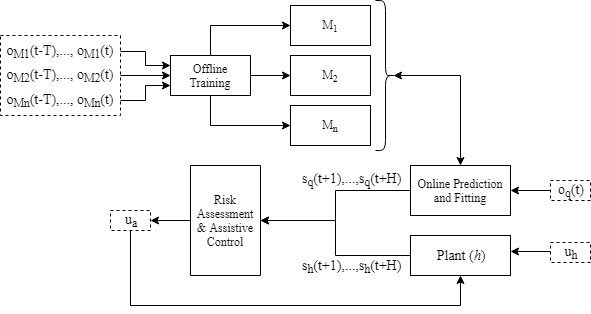
\includegraphics[width=0.48\textwidth]{approach.png}
    \caption{Block Diagram of the Approach}
    \label{fig:app}
\end{figure}
\NB{let's revise this figure and add what I showed in the board yesterday}
%\NB{figure is too blurry}
%\NB{that's not a pictorial representation, It's a block diagram.}
%\NB{By using offline training we extract different models representing different vehicle behaviors. These models are then used online to .....}
Our approach, shown in Fig.~\ref{fig:app}, has the following components: We use offline training we extract different models representing different vehicle behaviors. These models are then used online to to predict future states of other vehicles, $\{s_q(t+1),\ldots s_q(t+H)\}$ over time horizon $H$, thus inferring their behavior to better assess safety and intervene to avoid hazardous situations. We leverage a history of offline observations, $\{o(t-T),\ldots,o(t)\}$, to build different models, $\{M_1,\ldots,M_n\}$, that are used online to recognize and predict new vehicles' behaviors. Based on these predictions, we want to monitor whether our vehicle, $h$, could enter an unsafe state.
 based on the user input, $u_h$. 
 If such an unsafe action is detected, an autonomous control action, $u_a$, is deployed to assist and correct the user's intention. In the next sections, we will go over this framework, explaining in detail each block presented in Fig.~\ref{fig:app}.
 
\NB{be consistent and formal with symbols: variable should be italic, vector should be bold, matrices should bebold upper case etc }
%\NB{fix this}. %\NB{simplify}
 %\NB{this should go in the related work}.% In this work, we train multiple models offline over a horizon $T$, with training sets that capture the behaviors of vehicles \NB{what vehicles...this sentence is incomplete.} \NB{also you are repeating too many times the same thing and always not complete. This section should summarize what we are going to see next: using training data to predict future states and infer the behavior model of other vehicles, compare the prediction with our vehicle prediction to asses safety, monitor and intervene if needed by correcting behavior that can lead to unsafe situations}.

%\NB{In this work we train multiple models offline over an horizon {T}}

\section{HMM-based Training Framework} \label{sec:fmwk}
 In order to predict future states of other vehicles, we perform offline training of data collected over an horizon $T$ to extract and differentiate between different behavioral models. To this end, we propose a modified version of the Hidden Markov Model (HMM) \cite{woohmm} which can be described by a tuple $\langle \mathcal{O},\mathcal{S},\mathcal{E},\mathcal{G},\mathcal{P},\mathcal{B} \rangle$  where:
\begin{itemize}
    \item $\mathcal{O}\in\mathbb{R}^T$ is a finite set of observed states $o(t)$ collected over a finite past time horizon $T$, $\mathcal{O} = \{ o(t-T), o(t-T+1), \ldots, o(t)\}$. 
%    In our case $\mathcal{O}$ represent measurements about velocity and positions of surrounding vehicles
    %\NB{change to lower t}.
    \item  $\mathcal{S}\in\mathbb{R}^n$ is a finite set of $n$ unique values that $\mathcal{O}$ can obtain, i.e., $\{s_i,s_j\} \in \mathcal{S} \vert s_i \neq s_j$ with $i\neq j$,and $i,j = 1,\ldots,n$, with $n \in \mathbb{N}$.
    %\NB{no curly brackets when listing counters and indices}
    %\NB{i is equal to OR??? and OR is different to j??? not mathematically correct} The notation $s_{ij}$ represents the state transition from $s_i$ to $s_j$.\NB{there are so many issues in this sentence.}
    \item $\mathcal{C}\in\mathbb{R}^T$ %\NB{what's the dimension of C?}
    is the finite set of emissions, or inferences $c(t)$ that relate to the action taken each state, and $\mathcal{C} = \{ c(t-T), c(t-T+1), \ldots, c(t)\}$. %\NB{what does it mean that it relates to each state? Explain better} $T$, 
    \item $\mathcal{G}\in\mathbb{R}^m$ is a finite set of $m$ unique inferences that $\mathcal{C}$ can obtain. and $g_k \in \mathcal{S}$, where $k = 1,\ldots,m$, with $m \in \mathbb{N}$. 
    \item $\mathcal{P}\in\mathbb{R}^{n\times n}$ is a transition probability matrix. This matrix describes the probability of entering a certain state, $s_{j}$, while currently in a particular state $s_{i}$, denoted as $s_j \to s_i$, defined by:
        \begin{equation}
            p_{ij} = P(s_j\to s_i)
        \end{equation}
        These probabilities are initialized as $1/n$. Each transition probability is calculated by counting the occurrences of each state transition over all transitions from that state:
        \begin{equation} \label{eq:transbuild}
            p_{ij} = N_{ij}/N_{i}*
        \end{equation}
        where $N_{ij}$ represents the total number of transitions, $s_j \to s_i$, over $T$ and $N_{i}*$ is the total number of transitions from $s_i$ to any state, and $N_{ij} \leq N_{i}* \leq T$. The state transition matrix is right-stochastic, meaning the sum of all rows is $1$ and is of the form:
        \begin{equation}
            \mathcal{P} = 
                    \begin{bmatrix}
                        p_{11} & \dots & p_{1n} \\
                        \vdots & \ddots & \\
                        p_{n1} &    & p_{nn}
                    \end{bmatrix}
        \end{equation}
    \item $\mathcal{B}\in\mathbb{R}^{n\times m}$ is the emission matrix, which lists the probability $b_{ik}$ of obtaining emission $g_k$ given state $s_i$:
        \begin{equation} \label{eq:obsref}
            b_{ik} = P(g_k(t+1) \vert s_i(t))
        \end{equation}
        where $i = 1,\ldots,n$. These probabilities are initialized as $1/m$, and are calculated in a similar way to (\ref{eq:transbuild}):
        \begin{equation} \label{eq:obsbuild}
            b_{ik} = N_{g_{ik}}/N_{g_{i}}*
        \end{equation} 
        where $N_{g_{ik}} \leq N_{g_{i*}} \leq T$.
        \begin{equation}
            \mathcal{B} = 
                    \begin{bmatrix}
                        b_{11} & \dots & b_{1m} \\
                        \vdots & \ddots & \\
                        b_{n1} &    & b_{nm}
                    \end{bmatrix}
        \end{equation}
 %       The matrices $\mathcal{P}$ and $\mathcal{B}$ will be referenced as ``the parameters" of the AHMM in the rest of this work. \NB{no let's use their name in the paper}
\end{itemize}

This framework is executed over $T$ and a set of parameters is obtained: $\langle \mathcal{P}, \mathcal{B} \rangle$. Our framework is different from a traditional HMM because the states are not hidden, and we know exactly the relationship %\NB{not sure about this and we should not add AHMM, We haven't defined it yet and it seems unnecessary to give a name to this unless we have really major changes to the way it computes states and transitions}
%\NB{clarify}
%with implicit parameters $m$ and $n$ \NB{this sentence is confusing}
between states and their corresponding inferences. Because we have all the states and transitions a priori, we can learn the parameters of multiple models offline. %In addition, having the knowledge pertaining to the relationship between states and inferences allows predictions to be made with increased accuracy.\NB{how? This sentence is telling everything and nothing}
The general pictorial representation of the AHMM is shown in Fig.~\ref{fig:hmm} %\NB{what's a in the figure?}\NB{figure needs improvement: make it smaller vertically...too much space in between s and c. Increase fonts}.
In this image, nodes labeled $s$ represent the states ($\mathcal{S}$), while those labeled $c$ represent the emissions ($\mathcal{C}$). The lines with the label $p$ represent the transition probabilities between states, and those labeled $b$ represent the probability that each of the connected observations are associated with connected states.

\begin{figure}[ht!]
    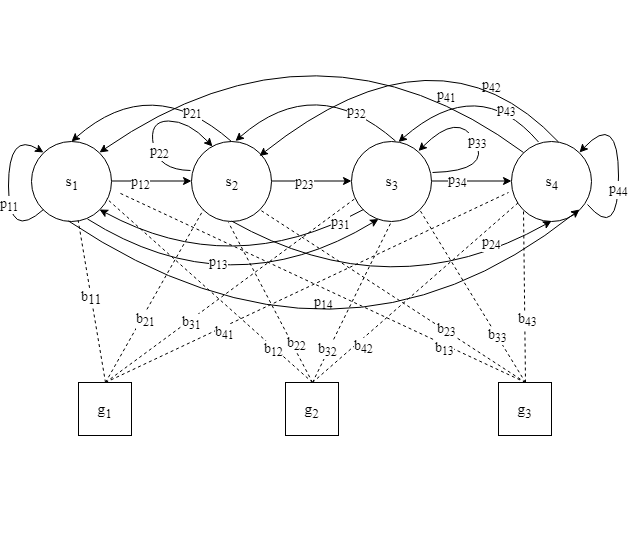
\includegraphics[width=0.48\textwidth]{ahmm.png}
    \caption{General Representation of an Adjusted Hidden Markov Model. In this figure, states, emissions, and respective transition and emission probabilities are shown.}
    \label{fig:hmm}
\end{figure}

The specific environment we are studying involves multiple lanes with multiple vehicles that can change their velocities and their lanes. Within this environment, we are able to set up two AHMMs to capture the behaviors we expect to see. The AHMMs are applied to all of the vehicles, $q$ in our sensing range $R$.

The two AHMMs will aim to predict future velocities $v$ and lanes $l$ of the vehicles. In this model, $S_v = \{v_1,\ldots, v_n\}$, $S_d = \{d_1,\ldots,d_n\}$,$S_l = \{l_1,\ldots,l_n\}$, where $S_v$ is the set of velocities, $S_d$ the set of distances between vehicles, $S_l$ is the set of lanes. The emissions reflect the actions performed between two consecutive states. In our case, emissions are the inputs to vehicles that we are most concerned with; changes in velocity and changes in lane. %\NB{let's discuss that these emissions are the inputs that we care i.e., changes in speed and changes in lanes}
For velocity we consider the following 3 emissions,
    
%\NB{too many words...$S_v$ is the set of velocities and $S_d$ the set of distances between vehicles}

\begin{itemize}
    \item[$b_1^v$] {Increasing Velocity if $v(t) > v(t-1)+\delta_v$} 
    \item[$b_2^v$] {Decreasing Velocity if $v(t) < v(t-1)-\delta_v$}
    \item[$b_3^v$] {Maintaining Velocity if $v(t-1)-\delta_v \leq v(t) \leq v(t-1)+\delta_v$}
\end{itemize}
%\NB{formalize...$v(t-1)+\delta_v$ etc}
%\NB{give a name to this emissions...i.e. $b_{1}^v, b_{2}^v$}
%\NB{if not where}


For the lanes, the following 3 emissions are considered:

\begin{enumerate}
    \item[$b_1^l$] Changing Left if $l(t) < l(t-1)$
    \item[$b_2^l$] Changing Right if $l(t) > l(t-1)$
    \item[$b_3^1$] Not changing if  $l(t) = l(t-1)$
\end{enumerate}
where we assume that lanes are modeled in increasing order from left to right; i.e. the leftmost lane is $1$ and the rightmost lane is $n$.
%\NB{what does it mean $lane < lane$?}
%\NB{same as before...formalize this}
%\RP{capture that the emission are related to actions}


\section{AHMM-Based Online Prediction and Model Updates} \label{sec:ahmmpredupdate} %\NB{perhaps combine with next and add Update in the title}
  Using the HMM approach outlined in Section \ref{sec:fmwk}, given enough observations, we can extract a model for each surrounding vehicle. This model can be used online to predict future states of the system, and this is achieved by collecting more observations online. These online observed states can then be applied to the available, previously collected emission and transition matrices as lookup tables to obtain the most likely future state. The future state is determined using:
 %\NB{Using the HMM approach outlined in Section...given enough observations, we can extract a model for surround vehicles}. \NB{This model can be used online to predict future states of the system. This is achieved by collecting more observations online. The observed states at time t can then be used in the available emission and transition matrices, as a lookup table, to obtain the most likely next state}At $t$, the parameters of the AHMM can be used to make online predictions about the future states of the observed system. This is done by identifying the current state, $s_{i}(t)$ and applying it to the transition and emission matrices, which are used as lookup tables, to obtain the next most likely state and its likelihood. %We start with the assumption that $\mathcal{P}$ will give conclusive results from which we can predict the future state as follows\NB{remove this}:
%\begin{equation} \label{eq:nextstate}
%    s_{i}(t+1) = \max_{j}[\mathcal{P}_{i(t),j}]
%\end{equation}
%\NB{this equation is wrong. a state is not equal to the probability!}
%There is, however, the possibility that there will be more than one returned states, as the maximum transition probability %can be the same for multiple states. In this situation, we invoke the use of $\mathcal{B}$:
%\begin{equation} \label{eq:nextemis}
%    g_{k}(t+1) = \max_{k}[\mathcal{B}_{i(t),k}]
%\end{equation}
%\NB{this should be only between the two that are uncertain and that formula is not resolving the issue! }
%\NB{equation needed}.
\begin{equation} \label{eq:pred}
   s(t+1) = s_j \in S \vert p_{ij}=\max(\mathcal{P}_i)
\end{equation}

In the event that \eqref{eq:pred} returns more than one value, we cross-reference the states with the emission matrix, $\mathcal{B}$ as follows: 
\begin{equation} \label{eq:pred2}
    s(t+1)=s_j\vert g_{ij} = \max(\mathcal{B}_i)    
\end{equation}

%\NB{s(t+1) doesn't return multiple values....if there are multiple states that satisfy equation 13. You should go to another line and state that not in an equation environment}
%\NB{change the symbol for and. I'm also not 100\% sure that this expression is correct}
%Because the relationship between states and observations is not hidden, we can use the expected inference, derived from \eqref{eq:pred} to assess which returned state is more accurate \NB{not clear, rewrite}.

In the event that \eqref{eq:pred2} still returns more than one state, we choose the more dangerous transition, which depends on the specific application. For instance, in our case, the more dangerous transition is one that minimizes the distance between our user's vehicle and the observed vehicle.
%\NB{go to another line}

Using this approach, we can predict a series of future states over any horizon $H$ by assuming that each prediction for $t+1$ is correct. We re-use the emission and transition matrices to predict next state at $t+2$ and so on, up to horizon $H$. It is, however, important to note that as $H$ is increased, every successive prediction tends to be less accurate, as the sequence of future predictions is built assuming each of the previous predictions is correct.
%\NB{flip the order} \NB{explain the algorithm}.
Algorithm\ref{alg:pred} shows how we carry forward this prediction through $H$.%\NB{fix this sentence}.\NB{summarized the steps...}
In this algorithm, an observed state, $s(t) = s_i$, is used in %\NB{in not with} 
$\mathcal P$ and $\mathcal B$ to find the most likely next state, $s(t+1) = s_{j^*}$ %\NB{$s_j^*$}.
The following state, $s(t+2)$ is calculated using the previously determined $s_{j^*}$, assuming that it is the next observation. This process is repeated up to $t+H$, such that we have an series $\{s(t+1),\ldots,s(t+H)\}$.
%\NB{I think we can remove this if you have explained the procedure well before}
%\NB{assuming that next observation is be the predicted $s(t+1)$}. This process is repeated up to $t+H$.

\begin{algorithm}[ht!]
\caption{Future State Prediction} \label{alg:pred}
\begin{algorithmic}[1]
\WHILE{$t\leq t+H$}
\STATE $s(t) = s_i$
\STATE $s(t+1) = s_j \in S \vert p_{ij}=\max(\mathcal{P}_i)$
\IF{$s_j$ is not a singleton, i.e. $s_j\in S'\in S$}
\STATE $s(t+1)=s_j\in S'\vert g_{ij} = \max(\mathcal{B}_i)$
\STATE $s(t+1) \gets s_{j}$
\IF{$s_j$ is not a singleton}
\STATE $s(t+1) = \max_{s_j}S'$
\ENDIF
\ENDIF
\STATE $s_i = s(t+1)$
\STATE $t \gets t+1$
\ENDWHILE
\end{algorithmic}
\end{algorithm}

%\NB{what's $\mathcal{P}_{i}*$? and $j*$...btw it should be $j^*$}
%\NB{this is not correct! The prediction is still not sure because we don't know what's going to happen. On the other hand we want to improve the prediction itself and thus we update the model online}.

It is, however, possible that the online predictions are incorrect, indicating that our model does not accurately represent the system we are observing online. In order to alleviate this issue, we propose a method to update $\mathcal{P}$ and $\mathcal{B}$ online. This is achieved by using \eqref{eq:transbuild} and \eqref{eq:obsbuild}, where we adjust $N_{ij}$ and $N_{ik}$, and therefore, $p_{ij}$ and $b_{ij}$ will change. As a result, new transition and emission matrices $\mathcal{P'}$ and $\mathcal{B'}$ are created at each iteration to reflect the updates. In addition, we use a sliding window approach such that the size of the training set is always a constant $T$. %\NB{is always constant $T$}\NB{remove this last part}.
The training set is kept the same size in order to retain computational efficiency and to avoid keeping older and less reliable data. Another option would be to discount older data, however we decide not to use this method in this paper because the transition and emission matrices will grow larger, decreasing the efficiency of the proposed method. 
%$\mathcal{P'}$ and $\mathcal{B'}$ are updated each iteration and will continue to be used for online prediction, making each prediction up-to-date with the online observations. \NB{this last part need to be revised} %\NB{rewrite} %\NB{simplify}

\section{Online Model Fitting}\label{sec:omf}
Using the framework described in Sections \ref{sec:fmwk} and \ref{sec:ahmmpredupdate}, we can extract a model that captures the behavior of a system that we have been observing for $T$. Multiple models can be extracted using several data sets, and with that we can obtain super-sets containing all the transition and emission matrices for multiple vehicles. It is important to note that these models capture different behaviors, and we assume that we have enough different models to fit any new system during run-time. $\mathcal{M} = \{M_1,\ldots,M_m\}$ is the set of $m$ models. %\NB{too many words...M  is the set of m models.}.
The transition and emission matrices of these models are denoted as follows: %\RP{reorder later} %\NB{here we should probably remind the reader that these models capture different behaviors and we assume that we have enough behaviors to model any system during run-time. This concept should be clear also in the introduction}: 
\begin{equation}
    \hat{\mathcal{P}} = \{\mathcal{P}_1,\ldots,\mathcal{P}_m\}
\end{equation}
\begin{equation}
    \hat{\mathcal{B}} = \{\mathcal{B}_1,\ldots,\mathcal{B}_{m}\}
\end{equation}

%\NB{where $M\in\mathbb{N}$ represents the number of models}.

During run-time we observe new measurements of other vehicles. The challenge here becomes fitting each vehicle's observations to the right model computer offline. However, until we have enough observations, the prediction may not be accurate. Thus, we need to take into account possible errors in the prediction, $e$ as we are matching the vehicle behavior with the offline models. 

%In efforts to minimize situations where transitions are unclear, we propose training multiple models prior to the prediction process.\NB{??? What does this last sentence mean?} \NB{just say that we assume to have collected enough models offline to be able to fit and match any new vehicles that appear in our range}

%\NB{We treat any vehicle observed online as a new system and follow the approach outlined in Section...to obtain P and B. At each iteration P and B are updated and compared with the existing Models. The closest model is chosen to predict the behavior of the system. }Having built multiple models, we observe a new vehicle and begin to execute the framework discussed in Section \ref{sec:fmwk} for two consecutive measurements, $\left[o(t-1),o(t)\right]$. With this information, we are able to further execute the framework and determine parameters $\tilde{\mathcal{P}}$ and $\tilde{\mathcal{B}}$, which stand for the transition and emission matrices for the system we are currently observing. In order to determine the optimal model, we calculate the set of errors, $\hat{e}_{N_{M}} = \{e_{N_1},\ldots,e_{N_M}$\} between our model and each of the offline models:

We treat any vehicle observed online as a new system from which we are interested to compute a model, hence we follow the same procedure in Section \ref{sec:fmwk} to extract $\mathcal{P}$ and $\mathcal{B}$ and follow the approach outlined in Section \ref{sec:fmwk} to obtain $\tilde{\mathcal{P}}$, where $\tilde{\mathcal{P}}\in\mathbb{R}^{n\times n}$ and each element is initialized at $\tilde{p}_{ij} = 1/n$, where $i,j = 1,\ldots,n$. We also obtain $\tilde{\mathcal{B}}\in\mathbb{R}^{n\times m}$, where each element is initialized at $\tilde{b}_{ik}= 1/m$, where $i = 1,\ldots,n$ and $k=1,\ldots,m$. At each iteration, these matrices are updated using the method discussed in \ref{sec:ahmmpredupdate}, and are then compared with those of the existing models, $\hat{\mathcal{P}}$ and $\hat{\mathcal{B}}$. The closest model is chosen to predict the behavior of the system. In order to do this, we calculate the error between each model, $\mathcal{P}_i$ and our current transition matrix, $\tilde{\mathcal{P}}$:

 %\NB{how are these matrices initialized? We need to show the initial expression of these matrices 1/n ...}
 
\begin{equation} \label{eq:pnorm}
    \forall{P_i} \in \hat{\mathcal{P}}: e_i = \lVert\tilde{\mathcal{P}}-\mathcal{P}_{i}\rVert_{2}
\end{equation}
%\NB{is it $\hat{e}$ that you are computing? or each element?}
%\NB{check again the expression before; there are a lot of things that are not defined or make little sense}\NB{also I think the l1 and l2 is not correct now. Please check and write the correct expression}
where $\hat{e} = \{e_1,\ldots,e_m\}$, and $i\in\mathbb{N}^m$. In \eqref{eq:pnorm}, we use the $l2$ matrix norm to return a scalar, which in our case, represents the error between transition matrices of the observed model and the offline models. %\NB{What's the l2 of a matrix? Is it a scalar or a vector?}

%\NB{revise this}
In order to determine the model with the lowest error, we find the model that minimizes $\hat{e}$,

\begin{equation}
    M^*=M_i\in\mathcal{M}\vert e_i = \min(\hat{e})
\end{equation}
%\NB{need to check variables here}
%\NB{add argmin}

and $M^*$ %\NB{i is a index not a model}
is the model with the least error,\NB{this is unnecessary. Say this before, above...we find the model $M^*$ that minimizes the error...} which indicates the confidence we have in said model. A higher error indicates more uncertainty that predictions we make will be correct. The model with the lowest error is the one we are most confident in, and therefore, use to make predictions. We refer to $\mathcal{P}_{i^*}$ and $\mathcal{B}_{i^*}$ in order to make predictions. The procedure to predict future states is shown in Algorithm~\ref{alg:pred}. %\NB{something is missing here...we should somehow associate the error to the confidence that we have in that model....bigger errors = more uncertainties. The question becomes what should we do if the error is large or if it is small?? The answer is in the trust. What does it mean to trust mroe or less?}


%\NB{merge with previous and change to explain better how new data are going to improve your model...}
%If the observed system, however, does not result in an $i^*$ with a low error, the model is updated using the method discussed in Section \ref{sec:ahmmpredupdate} \NB{what does it mean....very confusing}. Because we are attempting to fit the model, rather than build a new one, we have the advantage of having the baseline, the current $N_M^*$ \NB{what is this baseline?}. We are able to leverage the parameters of this model, by  updating $\mathcal{P}_{N_M^*}$ and $\mathcal{B}_{N_M^*}$ as we observe new transitions or make new inferences, much like how we obtain $\mathcal{P}'$ and $\mathcal{B}'$ in Section \ref{sec:ahmmpredupdate} \NB{again very confusing}. In this case, we obtain $\mathcal{P}'_{N_M^*}$ and $\mathcal{B}'_{N_M^*}$. These models can be used to make future predictions using Algorithm \ref{alg:pred}.\NB{this last part is really bad written}


\section{Assistive Control} \label{sec:adapt}


\subsection{Reachability Analysis}

In order to assess risk of collision we need to predict:
\begin{enumerate}[i.]
\item future states of the surrounding vehicles which are obtained by following the procedure outlined in Section \ref{sec:ahmmpredupdate} and
\item the reachable states of $h$ over the horizon $H$.
\end{enumerate}
In some of our current work, we are using Hamilton-Jacobi reachability analysis to predict future states of a system under uncertainties \cite{esen}. In this paper, we consider a simplified approach for reachability in which we assume that:
\begin{enumerate}[i.]
\item The vehicle can move to the adjacent lane in one time step $\delta t$ \label{ass:i}
\item future variations of velocity are bounded $v_h-\delta_v \leq v_h\leq v_h+\delta_v$, with $\delta_v>0$ \label{ass:ii}
\end{enumerate}
Assumption \ref{ass:i} is made in order to treat the situation as a worst case scenario, and assumption \ref{ass:ii} is made to reflect a physical limitation of vehicles.
Three reachable velocities are computed using:
\begin{enumerate} %\NB{t+1 not i}
    \item $v_h(t+1)=v_h(t)$
    \item $v^-(t+1)=v_h(t)-\delta_v$
    \item $v^+(t+1)=v_h(t)+\delta_v$
\end{enumerate} 
and $\hat{v} = \{v^-(t),v_h(t),v^+(t)\}$, which is a time-varying set that depends on the current velocity, $v_h(t)$. Future reachable positions can be easily computed as $x_h(t+i)=v(t+i)\delta t$ for each of the three aforementioned velocities. Reachable lanes are modeled as $\hat{l} = \{l_1,\ldots,l_n\}$, where there are $n$ lanes. 
%\NB{this set is time varying and depends on the current velocity}
\begin{figure}[ht!]
    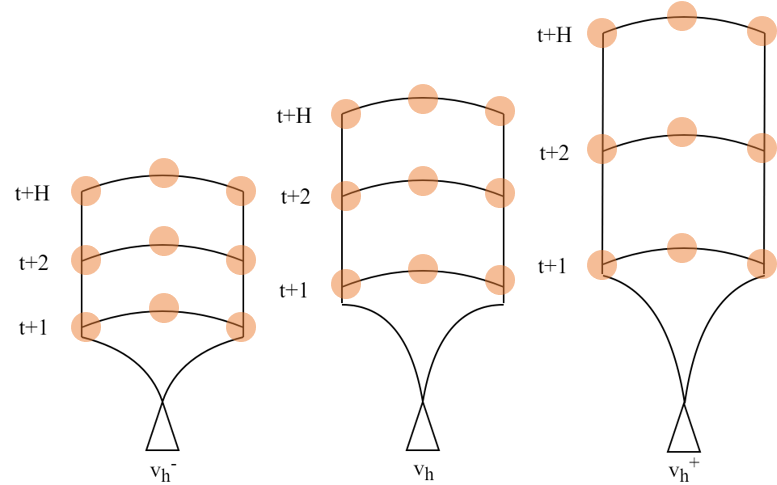
\includegraphics[width=0.48\textwidth]{input.png}
    \caption{Diagram of each reachable set}
    \label{fig:reach}
\end{figure}
%\NB{the iteration contains?}
Three reachable sets obtained contain the all the possible states that can be reached by $h$. For example if $h$ is on a 3 lane road and the prediction horizon is 3 time steps, assuming three velocity case above, then we obtain a total of 27 predictions, as indicated by the points in Fig. \ref{fig:reach}.
%\RP{dont forget to add picture}
%\RP{Predicting for H allows for trajectory generation for motion planning applications as well}

\subsection{Risk Assessment}

 In this section, we discuss how the our framework is used to guarantee safety for a HAV, $h$, over a time horizon $H$.
 
 %\NB{which vehicle? Any?}. In this situation \NB{what situation?}, we have our manned vehicle, $h$, and we have all of the vehicles in our vehicle's sensing range, $R_h$ \NB{$N_{R_h}$ vehicles are in range and can be monitored by $h$ \NB{remember to acknowledge that some vehicles may intermittently enter and exit the range of h}}:
 
 Risk is determined by computing the relative distance between $h$ and all vehicles $q\in R_h$ over the predictive horizon $H$, and $q\in\mathbb{N}^m$ where $m$ is the total number of vehicles in the sensing range.
 %\NB{and what? What's the solution here? }

%These vehicles will be referred to as agents in the rest of this work \NB{why??? What's wrong with vehicles? Please remove}.

By using the prediction approach presented in Section \ref{sec:ahmmpredupdate} we can predict future states for all $q$ over an finite horizon $H$ to obtain:
%\RP{Change to bar or tilde or hat for predictions}
\begin{equation}
    V_q = \{v_q(t+1),\ldots,v_q(t+H)\}
\end{equation}
\begin{equation}
    L_q = \{l_q(t+1),\ldots,l_q(t+h)\}
\end{equation}

%\RP{put in text}

where $V_q\in S_v$ and $L_q\in S_l$ are the predicted future velocities and lanes for each vehicle $q$, respectively.
With the future velocities, we are able to calculate the forward positions over the horizon $H$ using %\NB{what you mean the position for the horizon? } using %\NB{no need to use the $\forall$ here}: 
\begin{equation} \label{eq:dumpos}
    x_q(t) = v_q(t)\delta_t
\end{equation}
where $v_q\in V_q$ and $\delta_t$ refers to a sampling time. Using \eqref{eq:dumpos} we obtain future forward positions:
\begin{equation}
    x_q^p = \{x_q(t+1),\ldots,x_q(t+H)\}
\end{equation}
Using this information, we are able calculate relative distance,
\begin{equation}
    \forall q \in R_h: d_q(t) = \lVert x_h(t)-x_q(t)\rVert
\end{equation}

%Generating and using the optimal model for each vehicle $q$, as discussed in Section \ref{sec:omf}, we are able to predict where an agent will be in the environment for the user-defined time horizon, $H$, as discussed in Section \ref{sec:ahmmpredupdate}\NB{this sentence is confusing: By using the prediction approach presented in Section...we can predict future states for $q$ over an finite horizon $H$. }. This time horizon defines how far ahead the user wants the system to check, in order to intervene \NB{remove}. A sequence of future states for agent $q$, both in terms of velocity and lateral position, are developed for $H$ using the AHMM parameters and Algorithm \ref{alg:pred} \NB{merge this with the previous section}. Given a sequence of future predicted velocities,


%In this case, we also assume that the driver will continue the behavior he/she is doing at $t$ up to $t+H$. With this assumption, we are able to the estimate the future positions of $h$, obtaining the set:
%\begin{equation}
%    x_h^p = \{x_h(t+1),\ldots,x_h(t+H)\}
%\end{equation}

%\RP{Simplify - Risk is a function of D as follows}
Risk is a function of $d_q(t)$ and $l_q(t)$ %\NB{and the lane}
such that risk increases as distance decreases and as lane separation decreases and is calculated as follows: %\NB{what about the lanes?}

\begin{equation} \label{eq:riskcalc}
    r_{q}^{l}(t) =
    \begin{cases}
    \frac{1}{d_{q}(t)},  & \text{if } l_h=l_q \text{ and } d_{q}(t) > 1  \\
    \frac{1}{\xi d_{q}(t)},  & \text{if } l_h\neq l_q \text{ and } d_{q}(t) > 1  \\
        1,                     & \text{otherwise}  
    \end{cases}
\end{equation}

where $\xi$ is a function of the lane separation \NB{what is this function?}, and $r_{q}^{l}(t)$ represents the risk associated with vehicle $q$, evaluated at lane $l$ at time $t$. The values obtained from \eqref{eq:riskcalc} are calculated for each reachable velocity and position of vehicle $h$. The risk values are arranged as follows: %\NB{the vehicle are arranged as follows?}:

\begin{equation} \label{eq:riskmat}
\mathcal{R}_{q}^{v}=
\begin{bmatrix}
r_q^{l_1}(t+H) & \dots & r_q^{l_n}(t+H) \\
\vdots & \ddots & \\
r_q^{l_1}(t+1) &    & r_q^{l_n}(t+1)
\end{bmatrix}
\end{equation}
%\NB{what you mean interfering?}
where $q = 1,\ldots,m$ and $v\in\hat{v}$ and $\mathcal{R}_q^v\in\mathbb{R}^{H\times{n}}$. The matrices obtained from \eqref{eq:riskmat} build the superset $\mathcal{R}$ as follows:

\begin{equation} \label{eq:superrisk}
\mathcal{R} =
\begin{bmatrix}
\mathcal{R}_{1}^{v^-} & \ldots & \mathcal{R}_{m}^{v^-} \\
\mathcal{R}_{1}^{v} & \ldots & \mathcal{R}_{m}^{v} \\
\mathcal{R}_{1}^{v^+} & \ldots   & \mathcal{R}_{m}^{v^+}
\end{bmatrix}
\end{equation}
The representation in \eqref{eq:superrisk} suggests that multiple vehicles affect risk in our analysis. However, we are most concerned with the highest risk at each reachable point, which is evaluated as follows %\NB{any reachable point shown in Fig.}.
\begin{equation}
 \hat{\mathcal{R}}_{ij} = \max\begin{pmatrix}
 \begin{bmatrix}
\mathcal{R}_{1,ij}^{v^-} & \ldots & \mathcal{R}_{m,ij}^{v^-} \\
\mathcal{R}_{1,ij}^{v} & \ldots & \mathcal{R}_{m,ij}^{v} \\
\mathcal{R}_{1,ij}^{v^+} & \ldots   & \mathcal{R}_{m,ij}^{v^+}
\end{bmatrix}\end{pmatrix}
\end{equation}
%\NB{what's L? Define every variable, vector, set, etc...be careful that you may have already defined this before in another way}

%\NB{$\hat{r}_{v_h}$ is one value if I have to look this expression. why???}
 where $i = 1,\ldots,H$, $j = 1,\ldots,n$, and $\hat{\mathcal{R}} \in \mathbb{R}^{H\times n}$, where $H$ is the length of the time horizon and $n$ is the number of lanes.
 
 %Using \eqref{eq:lanerisk}, we obtain a distribution of all of the highest risk values for velocity $v_h$. % \NB{how are you combining these risks in one risk?}. 
 In Fig.~\ref{fig:riskd}, we show an example of a risk distribution, or $\hat{\mathcal{R}}$, over $H=3$ (left) for velocity $v_h$ at a the road scenario depicted (right).
 


\begin{figure}[ht]
    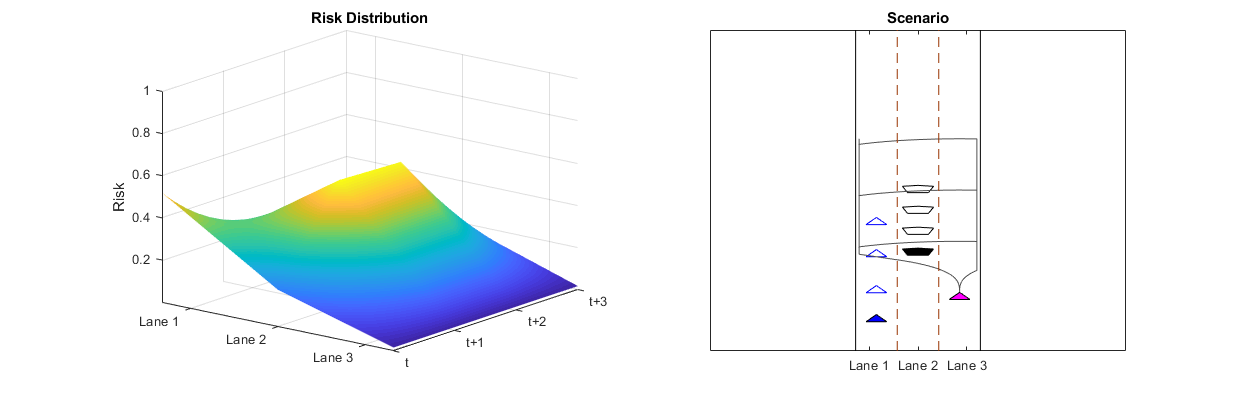
\includegraphics[width=0.48\textwidth]{assist.png}
    \caption{The distribution of risk at $v_h$ with $H = 3$ (left) for a certain road scenario (right). The magenta shape is the user's HAV, while the blue and black shapes are the actual positions of other vehicles on the road. Unshaded/outline shapes are predictions for vehicles in successive order; $[t+1,t+H]$. The lines coming out of the user's HAV are a visual depiction of the reachable set at the current velocity $v_h$.}
    \label{fig:riskd}
\end{figure}


%\NB{as mentioned during last meeting use solid filled shapes to show the current position and empty shape (not necessary to have a dashed line) for future states. No need to paint future states with different colors, just use the same color that you used to paint the shape of the vehicle. i.e., if the car on your left is blue, the future states are also blue}
%\NB{avoid this notation, this what?}

%\begin{equation}
%    \hat{\mathcal{R}} = \{\hat{r}^{L},\hat{r}^{C},\hat{r}^{R}\}
%\end{equation}
%\NB{this doesn't say too much. We can remove it probably}

\subsection{Adaptive User Assistance}

%\NB{define dangerous condition}
%\NB{...we propose a policy...}

Given the risk distributions, we can assist our user's potentially unsafe actions to guarantee safety, by performing actions that minimize risk. In order to adapt, we need to first identify whether these actions are going to result in a dangerous situation, or in this case, a collision. User actions, in this case, are limited to selecting a reachable lane and velocity,

\begin{equation}
u_h = (l_h,v_h), \text{ where } l\in\hat{l}, v_h\in\hat{v}
\end{equation}

A user-set threshold, $r_\max$ is used as a limit for risk \NB{what does it mean? A limit for risk for what? Be clear}. Given $r_\max$ and the values in the risk distribution for each velocity, as indicated in Figs.~\ref{fig:reach} and \ref{fig:riskd}, our system intervenes as follows:
\begin{equation} \label{eq:inputctrl}
    u = \begin{cases}
    u_h & \text{ if } \nexists~\hat{\mathcal{R}}_{ij} > r_\max \\
    u_a & \text{ if } \exists~\hat{\mathcal{R}}_{ij} > r_\max
    \end{cases}
\end{equation}
\NB{this is not what we are implementing...you are looking if any risk between now and H is above the maximum: if yes you switch to autonomous and send the vehicle toward the lane and velocity with the minimum risk associated}
%\NB{we need to define what are the inputs in our system}
where $u_a$ and $u_h$ represent autonomous and human inputs, and $u$ is the input to the vehicle $h$ \NB{super confusing. You should simply say that the input $u$ is going to be either the user input or the autonomous input as follows...and then show the equation above.}. During run-time, we are monitoring $r(t+1),...,r(t+H)$ in order to find the appropriate pair of actions (velocity and lane) for $t+1$ that minimizes risk $r(t+H)$, in the event that $r(t+H)\geq r_\max$ \NB{fix this}. We compute this pair by identifying the velocity and lane that produce the lowest risk based on our risk distributions $\hat{r}_v$:
\begin{equation} \label{eq:optlane}
    l^* = l_i\in\hat{l}\vert l_i = \argmin_{l}(\hat{r})
\end{equation}
\NB{so you pick the lane of the minimum risk even if the minimum risk is on t=3?} \NB{you should pick the lane such that the risk on that lane and for the next iteration is minimized.}
%\NB{what is the dimension of $\hat{r}_q^l$? From (22) it's one value} \NB{Why argmin with respect to $l_i$ and not $l$? Is it just $l_i$?}\NB{this expression is not correct! You need to pick the l and v associated to the minimum risk!}
\begin{equation} \label{eq:optvel}
    v_h^* = v_h\in\hat{v}\vert v_h = \argmin_{v_{h}}(\hat{r})
\end{equation}
\NB{what do you mean that you are picking $v_h$? What about if you have $v_h^-$ that is the best one?}
%\NB{what do you mean that you pick the minimum lane and velocity??? Please critique each expression that you write on the paper}
In a situation where $u = u_a$, as defined in \eqref{eq:inputctrl}, the input to the HAV is the optimal lane and velocity as indicated by \eqref{eq:optlane} and \eqref{eq:optvel}. The optimal lane and velocity are chosen such that the $r(t+H)$ is lowest for the reachable set that pertains to $(l^*,v_h^*)$, meaning that these inputs are determined to have the lowest $r(t+H)$ between all reachable velocities, $\hat{v}$ and lanes, $\hat{l}$. It is important to note that the risk is considered from $r(t+1),\ldots,r(t+H)$, meaning that if $r(t+H)\leq r_\max \land r(t+H-1)\geq r_\max$, the input is selected such that $r(t+H-1)$ is the risk we choose to minimize \NB{I'm confused on the approach}. By minimizing the most immediate high risk, assuming it is above the user's threshold, we are able to ensure that our input pair $u_a = (l^*,v^*)$ is always a safe action.  
[insert proof here where we prove that this always leads to the safest condition - we guarantee that the user action is guaranteed to produce a risk below the threshold. Show the math]


%Because the risk is calculated for each lane, the initial action is to identify if a certain lane has a lower risk. With this, we identify $l^*$, which is the lane with the lowest risk:
%\begin{equation}
%    l^* = \min_l(\mathcal{\hat{R}})
%\end{equation}
%In addition, we consider the fact that a lane change may be unavailable or unfeasible due to environmental constraints. In this case, we determine the minimum and maximum velocities our vehicle should be driving within one lane. In order to calculate these values, we first find a range $[d_{\min},d_{\max}]$ that our vehicle must be within, in order to ensure that the risk stays below $\rho$. After these safe distances are determined, a maximum velocity and minimum velocity are found such that this range is not violated for horizon $H$.
%\RP{1. if one of the vs is safe, then we do that}
%\begin{equation}
%    v_{\min} = d_{\min}/H
%\end{equation}
%\begin{equation}
%    v_{\max} = d_{\max}/H
%\end{equation}

% Let us take, for example, our host vehicle travelling at a much higher velocity than a preceding agent in the same lane. Our system identifies that our user has not shown any sign of turning, and because of that, we assume the user's priority is to stay in the lane. As a result of this, the $u_a$ involves lowering the velocity first. Assuming that the user doesn't respond, our system will continue to lower the velocity such that $u_s = v_q$, as long as the risk remains below $\rho$. If the user responds with a sub-optimal lane change, then the system will assist the user by reverting to the optimal action instead.  


\section{Simulations} \label{sec:sims}
The simulations for this work were done in Matlab. Different simulations were run for each part of the approach depicted in Section \ref{sec:approach}. We first discuss how the models were trained, and we validate those results for both velocity and lateral positions (lanes). This is followed by showing an example of fitting one model given multiple pre-trained models and a new system to observe. Lastly we demonstrate the risk estimates, and the assistance given to the user's actions, in order to verify that we are able to avoid risk of collision.

\subsection{Training Models}
In order to train the models, we used a workspace featuring $6$ stationary obstacles. A test vehicle drove through this workspace, while avoiding these obstacles, and it was observed for a training period of 700 iterations. In this period, the framework discussed in Section \ref{sec:fmwk} was executed and $\mathcal P$ and $\mathcal B$ matrices were generated. In order to validate the effectiveness of the generated matrices, we tested the sample over another period of the same length with $9$ obstacles. In verifying the results for velocity, we used forward position, which is calculated using the relationship in \eqref{eq:dumpos}. The resulting root mean squared error (RMSE) for forward position estimates was $1.3927$m. The results for velocity prediction are shown in Fig.~\ref{fig:train1}, where the validation begins after the vertical line labeled ``End Training Set". 

\begin{figure}[ht]
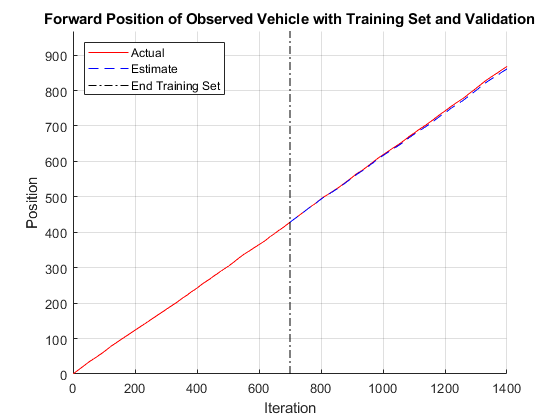
\includegraphics[width=0.48\textwidth]{train1.png}
\caption{The forward position of the actual vehicle (red) is shown. After the training set, a prediction is made and the forward position of the estimate is shown (blue dashed).} \label{fig:train1}
\end{figure}

In addition to velocity, we also measure the accuracy of our predictions regarding lane changes and following distances at which these changes occurred. Based on results shown in Fig.~\ref{fig:train2}, it is evident that the expected lane changes occurred, and to validate the following distances at which the lane changes took place, we used RMSE, which was $1.2564$m. The results for both velocity and lane change distance validation showed that the predictions were very effective when predicting the future states of the same model.

\begin{figure}[ht]
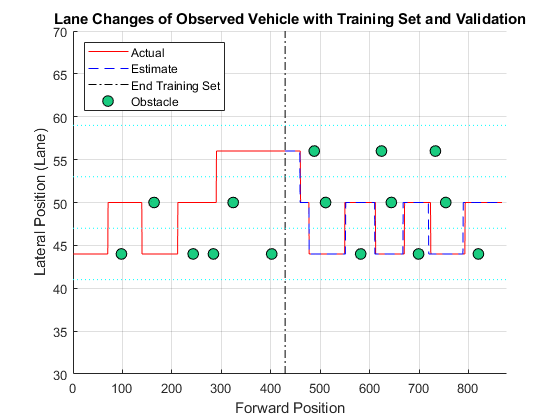
\includegraphics[width=0.48\textwidth]{train2.png}
\caption{The lane changes of the actual vehicle (red) are shown. After the training set, a prediction is made and the lateral positions/lane changes of the estimate is shown (blue dashed).} \label{fig:train2}
\end{figure}




\subsection{Fitting Models}

In this section, we show that we are able to fit pre-trained models to a new vehicle online. The behaviors of this vehicle are randomly generated and used to find the appropriate model. In order to determine the appropriate model, we use \eqref{eq:pnorm} with each of the three pre-trained models. We obtain and display the errors in Fig.~\ref{fig:error}.

\begin{figure}[ht]
    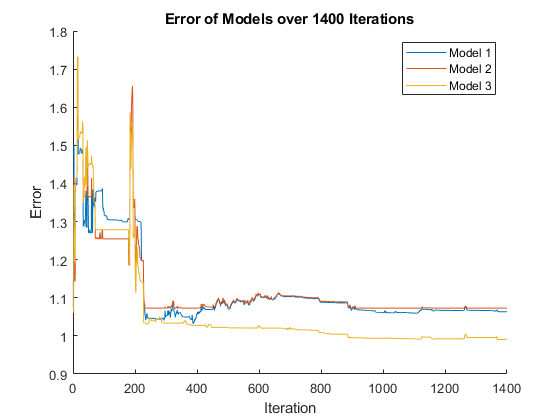
\includegraphics[width=0.48\textwidth]{modelerror.png}
    \caption{The error of the fit between our model and each of the three pretrained models} \label{fig:error}
\end{figure}

At each iteration, we use the model with the lowest error for future predictions. The selected model changes frequently at the start of run-time and converges to one model by the end of run-time. The selected model at each iteration is shown in Fig.~\ref{fig:select}. In this case, we converge to Model $3$ in approximately 300 iterations.

\begin{figure}[ht]
    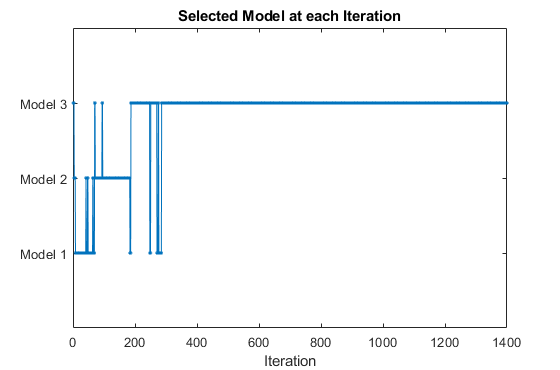
\includegraphics[width=0.48\textwidth]{modelselect.png}
    \caption{The error of the fit between our model and each of the three pretrained models} \label{fig:select}
\end{figure}

Using the selected model, we are able to make predictions for every iteration of run-time. In Fig.~\ref{fig:fwd}, we show the accuracy of the fit for velocity/forward position over 1400 iterations. The RMSE of this trial was $3.1423$m. In Fig.~\ref{fig:lanchan}, we show the the predictions made that pertain to lane changes and following distance. The RMSE of the predictions as compared to the actual actions was $3.5421$m. The RMSE values obtained for each of these tests suggest that the prediction is reliable. In addition, it was verified that the model chosen was the closest to the randomly generated behaviors, by examining the specific results of the randomization.


\begin{figure}[ht]
    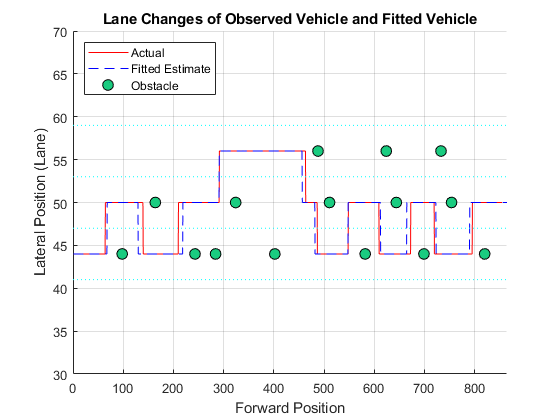
\includegraphics[width=0.48\textwidth]{fit2.png}
    \caption{The forward position of the actual vehicle (red) is shown. In addition, the forward position of the best-fit is shown (blue dashed).} \label{fig:fwd}
\end{figure}

\begin{figure}[ht]
    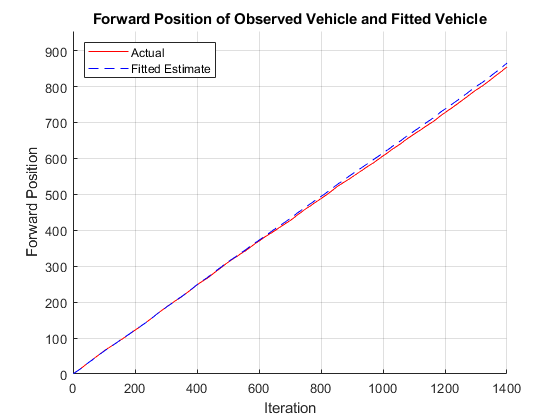
\includegraphics[width=0.48\textwidth]{fit1.png}
    \caption{The lane changes of the actual vehicle (red) are shown. The lane change predictions of the best-fit are shown (blue dashed).} \label{fig:lanchan}
\end{figure}
 
 

 
\subsection{Assistive Planning and Control}
In order to show the impact of our assistive control, we show a scenario where assistance is given to the user and one where it is not, and the user has full control of the HAV. In Fig.~\ref{fig:critpt}, we show a scenario where the risk, $r_h(t+H)$ at $H=3$ is surpassing the user set limit of $r_{\max} = 0.85$.


\begin{figure}[ht] 
    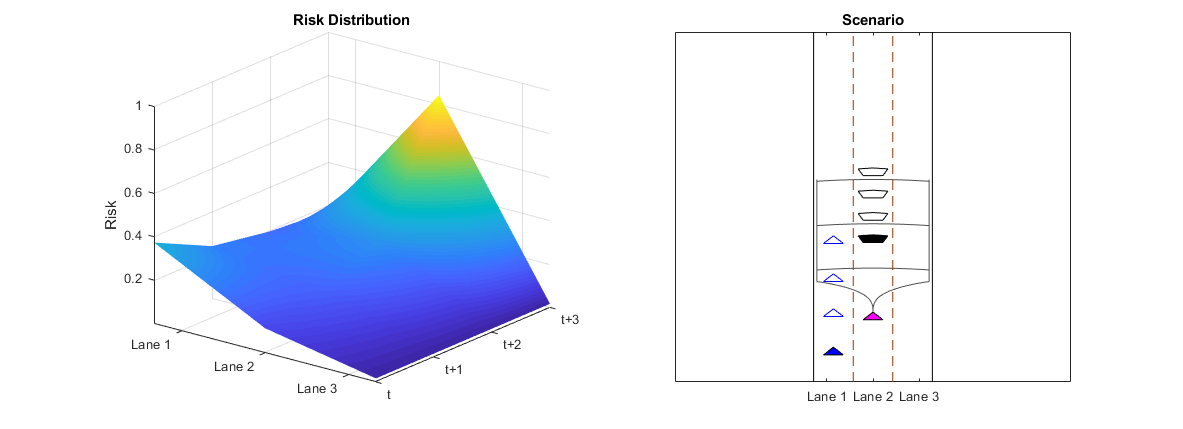
\includegraphics[width=0.48\textwidth]{critpt.png}
    \caption {In this snapshot, $r_h(t+H)$ is approaching $r_{\max}$. This is a situation where the HAV would assist the user in selecting the least risky action} \label{fig:critpt}
\end{figure}

In \ref{fig:critpt}, the magenta vehicle in the center is the HAV we are able to control. The reachable set is shown coming out of the HAV. In this case, we are only showing the reachable set and risk distribution for $v_h$. The snapshot occurs at a critical point, meaning a decision has to be made at this time, or a collision will occur in $H$. 


In Fig.~\ref{fig:noassist}, we show a scenario in which the user was unassisted. In this scenario, the user reached the same critical point as in Fig.~\ref{fig:critpt}, and decided to simply avoid the obstacle in front, indicated by the black polygonal shape, by moving to the left lane, unaware that an increased risk existed in the future for the left lane. In addition, the user did not adjust their velocity either, and as a result a collision occurred.

\begin{figure}[ht] 
    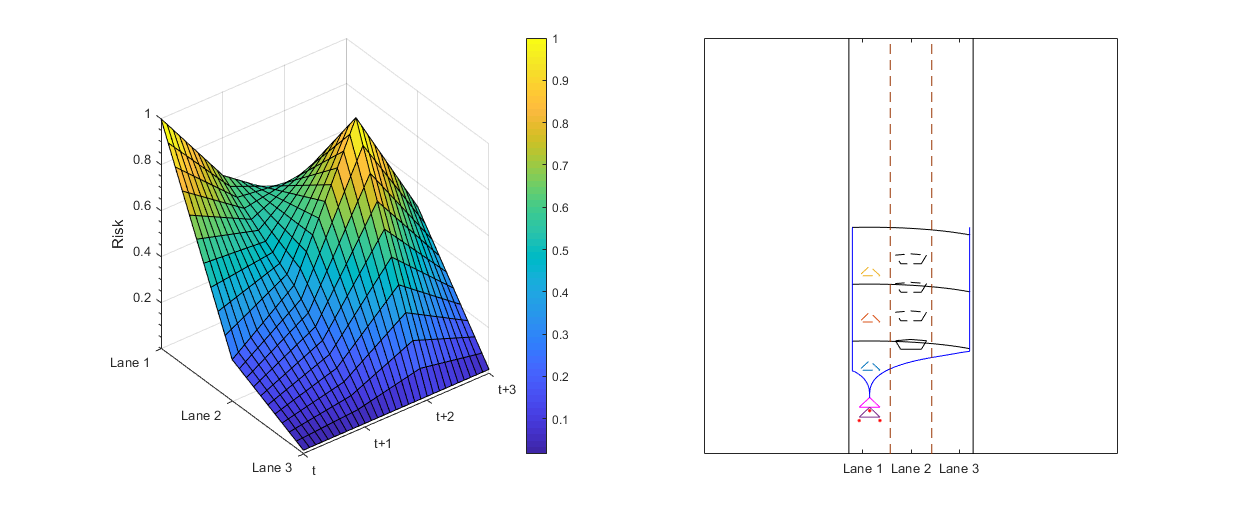
\includegraphics[width=0.48\textwidth]{noassist.png} 
    \caption{In this snapshot, a user has taken an unsafe action and it has resulted in high risk and a collision} \label{fig:noassist} 
\end{figure}

In Fig.~\ref{fig:assist}, we a show a scenario in which the user was assisted. The user input was modeled the same as in Fig.~\ref{fig:noassist}, but in this case, the assistive input was taken into account, as the risk surpassed $r_{\max}$. With assistive input, both lane and velocity were changed in order to minimize risk at every future time $t$ up to $t+H$.

\begin{figure}[ht] 
    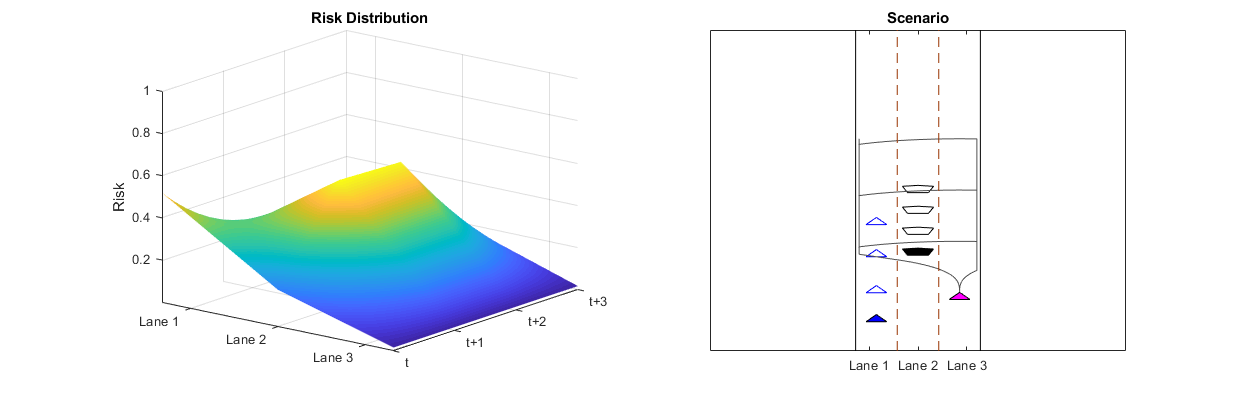
\includegraphics[width=0.48\textwidth]{assist.png} 
    \caption{This figure depicts a situation in which assistance has occurred and a risky situation was avoided altogether.} \label{fig:assist}
\end{figure}

 In the situation depicted in Fig.~\ref{fig:assist}, we are able to minimize risk and avoid collisions, thereby ensuring that our HAV is being operated safely.


\section{Conclusions} \label{sec:concs}
In this work, we have presented an approach for simultaneously predicting the future states of multiple vehicles and assisting the user of an HAV. Our approach uses a Hidden Markov Model based framework to build offline models of different vehicles and fit these models to any number of online observed vehicles. These models are used to make online predictions of the future states of the observed vehicles. We then use a simplified form of reachability analysis to ensure that the user of an HAV does not enter an unsafe state. The HMM based method for prediction is general across any type of system and the assistive control can be used for other vehicles, such as aerial vehicles and underwater vehicles.
\NB{KEEP THIS - this sentence needs more explanation. If we don't have enough models we need to mention that future work is centered on using existing models to extract new models}
% references section

% can use a bibliography generated by BibTeX as a .bbl file
% BibTeX documentation can be easily obtained at:
% http://mirror.ctan.org/biblio/bibtex/contrib/doc/
% The IEEEtran BibTeX style support page is at:
% http://www.michaelshell.org/tex/ieeetran/bibtex/
%\bibliographystyle{IEEEtran}
% argument is your BibTeX string definitions and bibliography database(s)
%\bibliography{IEEEabrv,../bib/paper}
%
% <OR> manually copy in the resultant .bbl file
% set second argument of \begin to the number of references
% (used to reserve space for the reference number labels box)

%\begin{thebibliography}{1}

%\bibitem{IEEEhowto:kopka}
%H.~Kopka and P.~W. Daly, \emph{A Guide to \LaTeX}, 3rd~ed.\hskip 1em %plus
%  0.5em minus 0.4em\relax Harlow, England: Addison-Wesley, 1999.
  
  
%\end{thebibliography}

%\printbibliography
\bibliographystyle{abbrv}
\bibliography{mybibliography.bib}


% that's all folks
\end{document}


